
%----------------------------------------------------------------------------------------
%	CHAPTER 2
%----------------------------------------------------------------------------------------
\chapterimage{chapter_head_2.pdf} % Chapter heading image

\chapter{Trabalhando o corpo}
\label{fig:bodyrelations}



%\begin{figure}[!h]
\begin{wrapfigure}{r}{0.5\textwidth}
\vspace{-10pt}
  \centering
    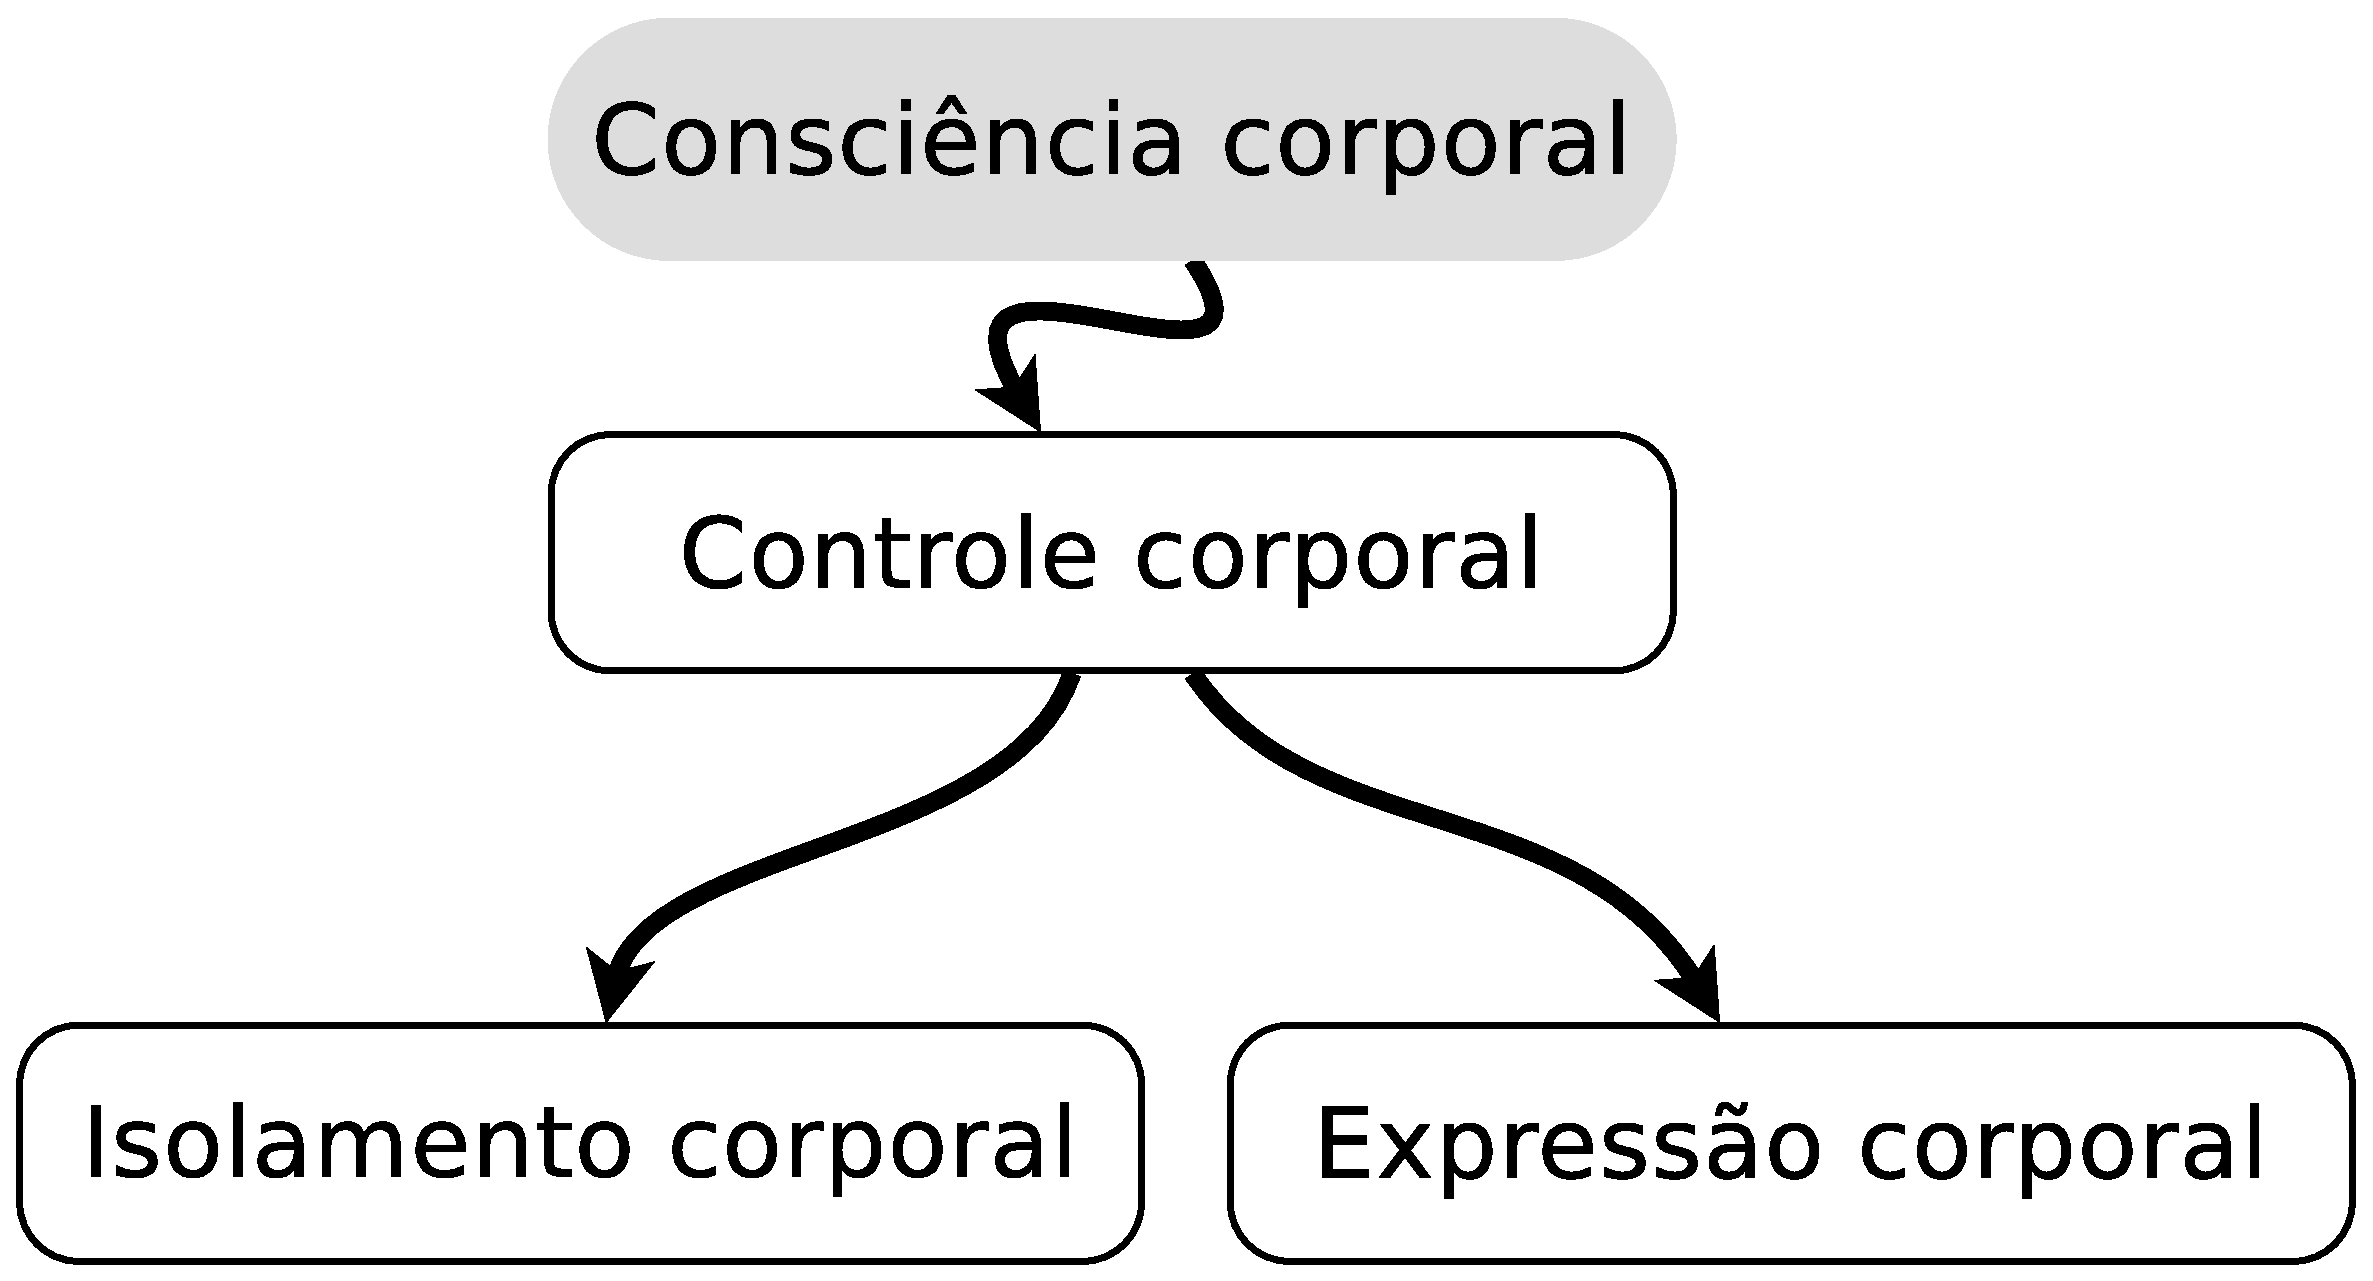
\includegraphics[width=0.475\textwidth]{chapters/cap-body/total.eps}
\caption{Trabalhando com o corpo.}
\vspace{-10pt}
\label{fig:bodycontroltotal}
\end{wrapfigure}
%\end{figure}
Quando dançamos a dois tentamos explorar e exteriorizar informações
provenientes de nosso mundo interior e o mundo exterior.
A informação interna corresponde à historia que queremos contar com nossa dança,
enquanto que a informação externa está dada pela música, nosso par de dança, e o entorno;
ainda assim, esta informação externa se expressa na dança 
mediante nossa própria interpretação da realidade.
Uma ferramenta indispensável para exteriorizar todas essas informações é o conhecimento e controle de
nosso próprio corpo, para conseguir isto existem alguns conceitos
como: 
a \hyperref[sec:BodyAwareness]{\textbf{consciência corporal}}, 
o \hyperref[sec:BodyControl]{\textbf{controle corporal}}, 
o \hyperref[sec:BodyIsolation]{\textbf{isolamento corporal}} e  
a \hyperref[sec:BodyExpression]{\textbf{expressão corporal}}.
A Figura \ref{fig:bodycontroltotal} mostra a relação de todos estes conceitos.


%%%%%%%%%%%%%%%%%%%%%%%%%%%%%%%%%%%%%%%%%%%%%%%%%%%%%%%%%%%%%%%%%%%%%%%%%%%%%%%%
\section{Que é a consciência corporal?}
\label{sec:BodyAwareness}
\index{Corpo!Body awareness}
\index{Corpo!Consciência corporal}
A consciência corporal, ou  ``Body awareness'' em inglês, 
tem sido estudada por diversos autores.
Seguindo a teoria de Wallon\footnote{Henri Wallon 
foi um célebre pedagogo que realizou estudos na área da psicologia infantil, 
cujas ideias foram plasmadas no livro ``A evolução psicológica da criança'' publicado em 1941.} 
é em torno aos 3 anos de idade que uma criança percebe, processa e reconhece
o que faz parte de si e sua relação com o exterior, é dizer, desenvolve a consciência corporal,
de modo que a percepção dos elementos do espaço antecede em muitos meses à 
percepção do próprio corpo e a relação com o mundo exterior
\cite{Garanhani2015} \cite{bueno2016psicomotricidade} \cite[pp. 154, 220]{wallon1968evoluccao}
\cite[pp. 14]{bolio2006fantasia},
isto tem sentido pois primeiro devemos ter o conhecimento que algo existe para 
depois ter a consciência de sua relação com nós e o mundo.
\begin{example}[Estudando nossa mão:]~

\begin{itemize}
\item Existe um objeto que chamarei mão, pois tenho detetado sua presença por meio do meus sentidos.
\item Tenho percebido que o objeto mão é parte de mim e com ela posso interagir com outros 
objetos. 
\end{itemize}
\end{example}
Por outro lado a consciência corporal também é descrita como a 
capacidade de uma pessoa em perceber a verticalidade do seu corpo 
(o eixo corporal \cite{bueno2016psicomotricidade}) de forma independente e 
sem referencias do exterior, 
de modo que a pessoa tenha uma união entre esquema corporal e imagem corporal \cite[pp. 14]{balcells2002expresion}.
\begin{example}[Passando por abaixo da mesa:]
Quando crianças aprendemos a reconhecer as partes de nosso corpo, dimensões, eixo e as relações com nosso entorno.
Um claro exemplo disso é quando uma criança passa por abaixo de uma mesa, 
pois estas, na maioria das vezes, tendem a agachar a cabeça ao passar 
devido a que sabem que sua altura real está 
um pouco acima da linha do seus olhos.
\end{example}

Uma habilidade necessária para ter a consciência do corpo é o ``esquema corporal'',
no qual a criança reconhece intelectualmente a existência das partes do seu corpo,
esteja esta em repouso ou em movimento
\cite{bueno2016psicomotricidade} \cite[pp. 24]{checa1999desarrollo}.
Outra habilidade é a ``imagem corporal'', 
a qual mostra como nos percebemos em relação ao mundo exterior,
nosso contexto e posição no espaço, esta é a forma em que nós representamos nosso corpo \cite[pp. 22-23, 27]{da2003imagem}.
Exemplo: Estamos sentados, estamos em pé ou deitados?.

\begin{tcbinformation}
\textbf{Consciência do par de dança:}
Podemos extrapolar o conceito de consciência corporal ao nosso par de dança,
pois da mesma forma que tomamos consciência de nossas dimensões, eixos, posição e postura no espaço,
é muito importante na dança a dois ter a consciência de estas caraterísticas em nosso par de dança
com o objetivo de melhorar nosso trabalho em equipo (``partnerwork'').
% Sensitivity to Others \cite[pp. 17]{paine2014complete}
% voce so deve souber onde está o um pé do par, não os dois, 
% vc deve de souber onde esta o pé que tem o peso do corpo,
% e imaginar a donde quer levar o pé livre.
\end{tcbinformation}

%%%%%%%%%%%%%%%%%%%%%%%%%%%%%%%%%%%%%%%%%%%%%%%%%%%%%%%%%%%%%%%%%%%%%%%%%%%%%%%%
\section{Que é o \bodycontrol?}
\label{sec:BodyControl}
\index{Corpo!Body control}
\index{Corpo!Controle corporal}

 O controle corporal ou ``body control'' em inglês, refere-se a capacidade
 de controlar as distintas partes de nosso corpo para realizar ações em nosso entorno, com eficiência e 
 mantendo o equilibro. 

Uma vez obtida a \hyperref[sec:BodyAwareness]{\textbf{consciência corporal}},
isto é, ter ideia do mundo interno e do mundo externo, 
o seguinte reto é conhecer nosso corpo a plenitude e dominar-lho, 
para obter este objetivo fazemos uso de nosso cérebro, sentidos, nervos, músculos, etc. 
não esquecendo nossos limites corporais e espaciais
\cite[pp. 14]{bolio2006fantasia}
\cite[pp. 27]{smith2011desarrollo},
por exemplo, o quanto podemos pular, quanto gira nossa articulação, onde termina meu espaço pessoal e inicia o espaço do próximo, etc.

De forma simplificada podemos dividir o controle corporal em controlador, equilíbrio e contração muscular;
o controlador seria nosso cérebro dirigindo todo o procedimento para obter um fim,
ele é consciente de nossa posição espacial, velocidade e nosso eixo (consciência corporal), 
controla e predize nosso comportamento; isto é possível graças a nosso equilíbrio,
que nos permite manter nossa postura atual em contra da força da gravidade e a inercia de nosso corpo em movimento;
para obter esse controle enviamos informação a nossos músculos para que tenham o 
tônus\footnote{O tônus muscular é o estado de tensão elástica do músculo em repouso,
este estado permite uma contração rápida quando é enviada pelo cérebro.
Se não existe tônus o músculo está relaxado,} adequado,
de modo que nosso corpo realize uma ação determinada em função da nossas necessidades
 \cite[pp. 17]{bolio2006fantasia}.
Ideias de como treinar nosso controle corporal podem ser vistas no Capitulo \ref{chap:trainingbodycontrol}.


\begin{tcbattention}
\begin{itemize}
\item Melhoramos nosso controle corporal mediante exercícios que requeiram
esticar e contrair os músculos com precisão relativa ao quando, o como e quanto, 
sem esquecer manter o equilíbrio.
Estes exercícios podem ser realizados com as pernas, os braços ou o corpo em geral.
\item Se melhoramos nosso controle corporal melhoraremos nosso uso de 
\hyperref[sec:musicalidade:dinamicas]{\textbf{dinâmicas}} na dança.
De forma reciproca, se melhoramos nossas dinâmicas teremos melhorado o controle de nosso corpo.
\end{itemize}
\end{tcbattention}
%%%%%%%%%%%%%%%%%%%%%%%%%%%%%%%%%%%%%%%%%%%%%%%%%%%%%%%%%%%%%%%%%%%%%%%%%%%%%%%%
\section{Que é o \bodyisolation?}
\label{sec:BodyIsolation}
\index{Corpo!Body isolation}
\index{Corpo!Isolamento corporal}


O isolamento corporal ou ``body isolation'' em Inglês é um termo utilizado
para descrever uma técnica usada na dança e áreas afins que 
consiste em mover uma ou várias partes ou eixos do corpo
de forma independente ou isolada do resto.
Para conseguir o isolamento corporal é necessário ter bem trabalhado nosso 
\hyperref[sec:BodyControl]{\textbf{controle corporal}} e a
\hyperref[sec:BodyAwareness]{\textbf{consciência corporal}},
e realizar treinamentos de dissociação das partes do corpo (dissociação corporal).
\index{Corpo!Dissociação corporal}
\index{Corpo!Movimento policêntrico}
\index{Corpo!Dança policêntrico}
Um termo equivalente ao isolamento corporal é dança policêntrica ou movimentos policêntricos,
que indicam movimentos com muitos centros de trabalho \cite[pp. 25]{grob2020dance}.

Os movimentos policêntricos são muito comuns nas danças com raízes africanas,
pois as músicas polirrítmicas tendem a gerar danças policêntricas;
nas danças atuais podemos ver esta caraterísticas na salsa, no samba de gafieira, no hip hop, o son cubano, entre outras
onde acharemos facilmente momentos em que uma parte de nosso corpo faz um trabalho
diferente em ritmo e movimento que o resto do corpo 
\cite[pp. 25]{grob2020dance} \cite[pp. 202-203]{madrid2013danzon} 
\cite[pp. 146]{dils2001moving} \cite[pp. 220]{antonacci2013memorias}.
Por exemplo, balanços de quadril e/ou ombros de forma isolada ao movimento de pés.
Ideias de como treinar o isolamento corporal podem ser vistas no Capitulo \ref{chap:trainingbodyisolation}.

%%%%%%%%%%%%%%%%%%%%%%%%%%%%%%%%%%%%%%%%%%%%%%%%%%%%%%%%%%%%%%%%%%%%%%%%%%%%%%%%
\section{Que é a expressão corporal?}
\label{sec:BodyExpression}
\index{Corpo!Body expression}
\index{Corpo!Expressão corporal}


\begin{wrapfigure}{r}{0.5\textwidth}
\vspace{-10pt}
  \centering
    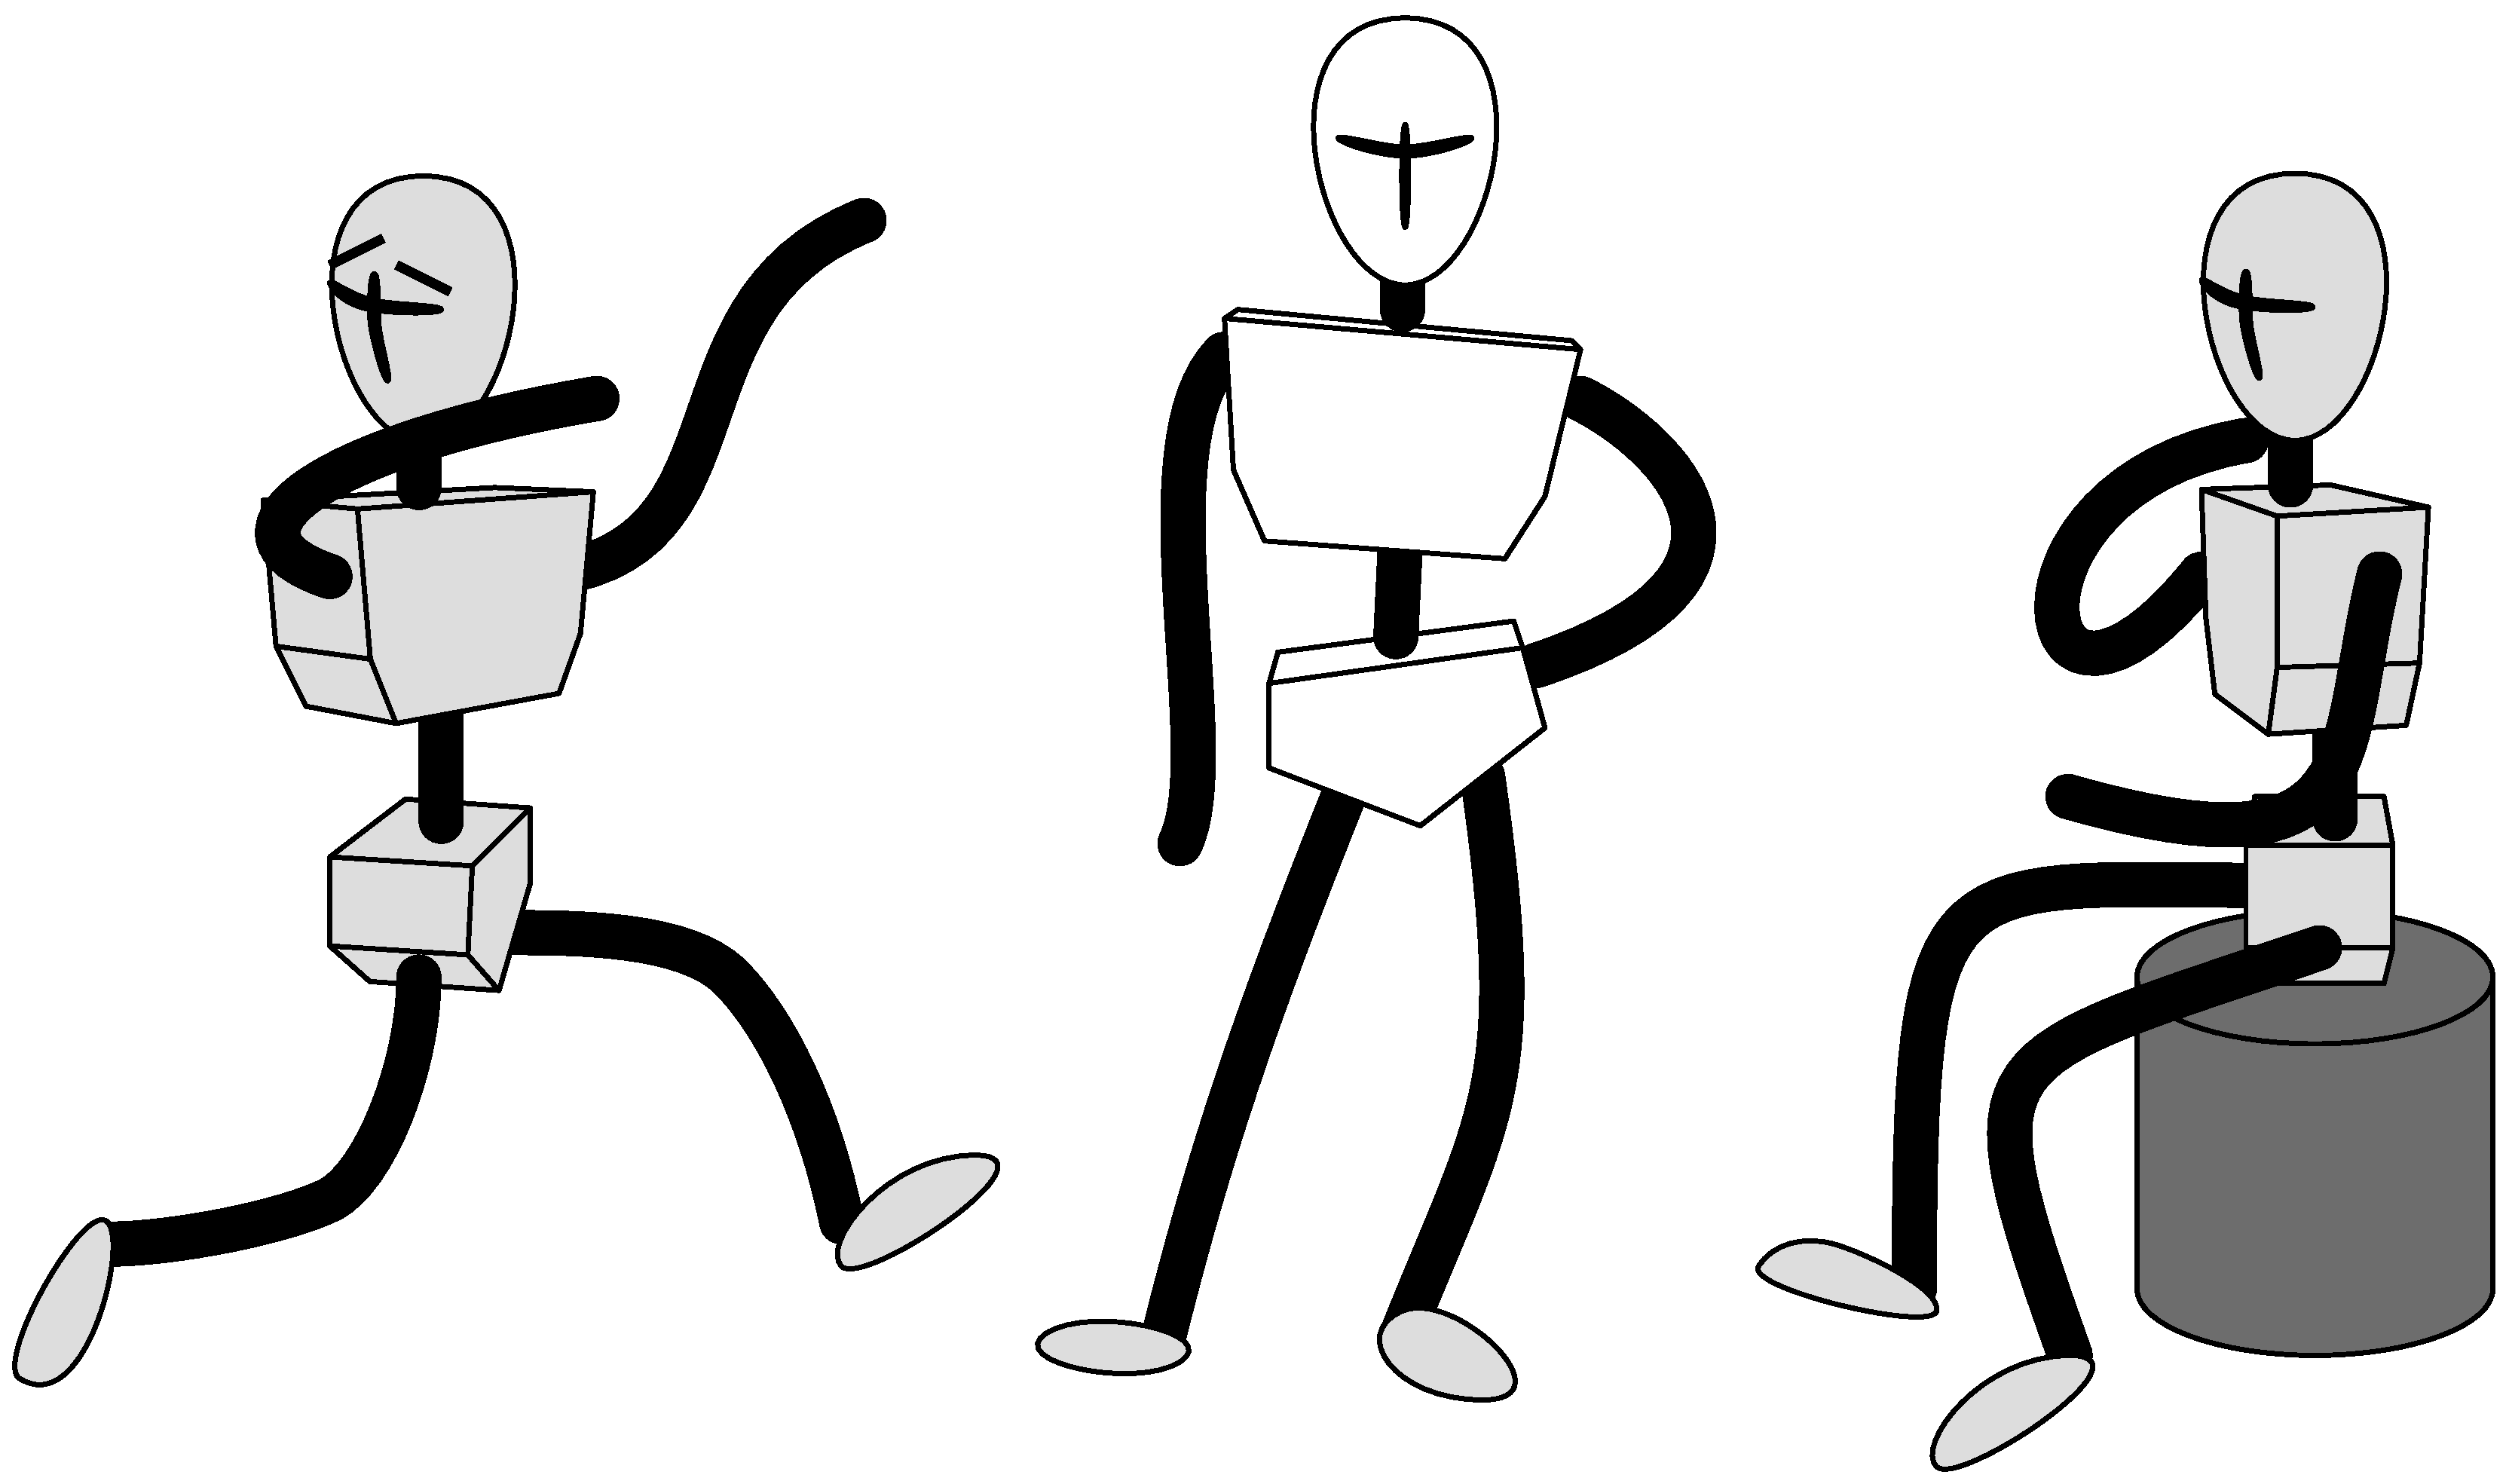
\includegraphics[width=0.475\textwidth]{chapters/cap-body/bodyexpresion-medo.eps}
\caption{Exemplos de expressão corporal.}
\vspace{-10pt}
\label{fig:bodyexpression1}
\end{wrapfigure}
A expressão é a manifestação do pensamento por meio da palavra ou do gesto.
Assim, a expressão corporal representa uma linguagem que estabelecemos através de nosso corpo,
já seja de forma estática ou em movimento  
\cite{bueno2016psicomotricidade} \cite[pp. 5]{balcells2002expresion},
esta linguagem está presente em distintas disciplinas como a danza, o teatro, mimo, entre outras 
\cite[pp. 5]{balcells2002expresion}.
A Figura \ref{fig:bodyexpression1} mostra alguns exemplos de expressão mediante o corpo.

A expressão corporal tem uma função importante na socialização dos indivíduos,
pois, além da comunicação oral e escrita, 
uma das formas mais básicas de comunicação realiza-se com o corpo das 
pessoas, mediante gestos, postura corporal, olhar, entre outros que conformam 
uma linguagem corporal \index{Corpo!linguagem corporal}
\cite{bueno2016psicomotricidade} \cite[pp. 6]{balcells2002expresion}.








